\documentclass{standalone}
\usepackage[dvipsnames]{xcolor}
\usepackage{tikz-network}

\definecolor{S}{HTML}{0b6884}
\definecolor{E}{HTML}{50b99a}
\definecolor{Ia}{HTML}{ff5e5b}
\definecolor{Is}{HTML}{ffc847}
\definecolor{R}{HTML}{7b678e}
\definecolor{D}{HTML}{bc4b51}

\definecolor{vuln}{HTML}{80475E}


\begin{document}
  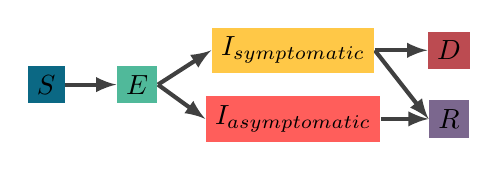
\begin{tikzpicture}[scale=0.66]
    \node at (-0.75, 0) (S) [shape=rectangle, fill=S] {$S$};
    \node at (1, 0) (E) [shape=rectangle, fill=E] {$E$};
    \node at (4,  0.66) (Is) [shape=rectangle, fill=Is] {$I_{symptomatic}$};
    \node at (4, -0.66) (Ia) [shape=rectangle, fill=Ia] {$I_{asymptomatic}$};
    \node at (7,  0.66) (D) [shape=rectangle, fill=D] {$D$};
    \node at (7, -0.66) (R) [shape=rectangle, fill=R] {$R$};

    \Edge[Direct](S.east)(E.west)
    \Edge[Direct](E.east)(Is.west)
    \Edge[Direct](E.east)(Ia.west)
    \Edge[Direct](Is.east)(R.west)
    \Edge[Direct](Is.east)(D.west)
    \Edge[Direct](Ia.east)(R.west)
  \end{tikzpicture}
\end{document}
